
\section{Auto MPG Dataset}

\subsection{Preprocessing: String Values, Missing Values, and Outliers}
\begin{itemize}
    \item \textbf{String Values:} The raw UCI file appends a 9th free-text field (car make/model, e.g.\ ``chevrolet chevelle malibu'') after the 8 numeric fields. This identifier column was dropped before regression since it carries no quantitative information; \texttt{origin} was kept as-is since it is already the standard numeric UCI code (1 = USA, 2 = Europe, 3 = Japan).
    \item \textbf{Missing Values:} The raw 398-row file contains 6 rows with \texttt{?} in the \texttt{horsepower} field (model years 1971, 1974, 1980, 1980, 1981, and 1982). These 6 incomplete rows were dropped (not imputed), yielding the standard 392-row, 8-column benchmark matrix.
    \item \textbf{Outliers:} Tukey's 1.5$\times$IQR rule flags 10 outliers in \texttt{horsepower} (bounds $[-1.5, 202.5]$, all above 202.5~hp) and 10 in \texttt{acceleration} (bounds $[8.9, 21.9]$). Flagged observations were retained to preserve the observed range; an IQR flag alone was not considered sufficient reason for deletion.
\end{itemize}

\subsection{Statistical Summaries for Each Feature/Variable}
\begin{table}[H]
\centering
\small
\begin{tabular}{lrrrrrrrrr}
\toprule
Variable & mean & std & min & 25\% & 50\% & 75\% & max & missing & outliers \\
\midrule
cylinders & 5.4719 & 1.7058 & 3.0000 & 4.0000 & 4.0000 & 8.0000 & 8.0000 & 0 & 0 \\
displacement & 194.4120 & 104.6440 & 68.0000 & 105.0000 & 151.0000 & 275.7500 & 455.0000 & 0 & 0 \\
horsepower & 104.4694 & 38.4912 & 46.0000 & 75.0000 & 93.5000 & 126.0000 & 230.0000 & 0 & 10 \\
weight & 2977.5842 & 849.4026 & 1613.0000 & 2225.2500 & 2803.5000 & 3614.7500 & 5140.0000 & 0 & 0 \\
acceleration & 15.5413 & 2.7589 & 8.0000 & 13.7750 & 15.5000 & 17.0250 & 24.8000 & 0 & 10 \\
model\_year & 75.9796 & 3.6837 & 70.0000 & 73.0000 & 76.0000 & 79.0000 & 82.0000 & 0 & 0 \\
origin & 1.5765 & 0.8055 & 1.0000 & 1.0000 & 1.0000 & 2.0000 & 3.0000 & 0 & 0 \\
mpg & 23.4459 & 7.8050 & 9.0000 & 17.0000 & 22.7500 & 29.0000 & 46.6000 & 0 & 0 \\
\bottomrule
\end{tabular}
\caption{Descriptive statistics for Auto MPG ($n=392$, $p=8$ columns).}
\end{table}

\subsection{Correlation Analysis: Matrix and HeatMap}
The full Pearson correlation matrix is printed by \texttt{xy.corr} in ScalaTion and \texttt{df.corr()} in Statsmodels/pandas; both agree exactly. Figure~\ref{fig:auto_mpg_heatmap} shows the heatmap (rendered via Statsmodels/seaborn; ScalaTion's \texttt{HeatMap} class from \texttt{scalation.mathstat} displays the identical matrix in an interactive window via \texttt{project1HeatMaps}).

\begin{figure}[H]
\centering
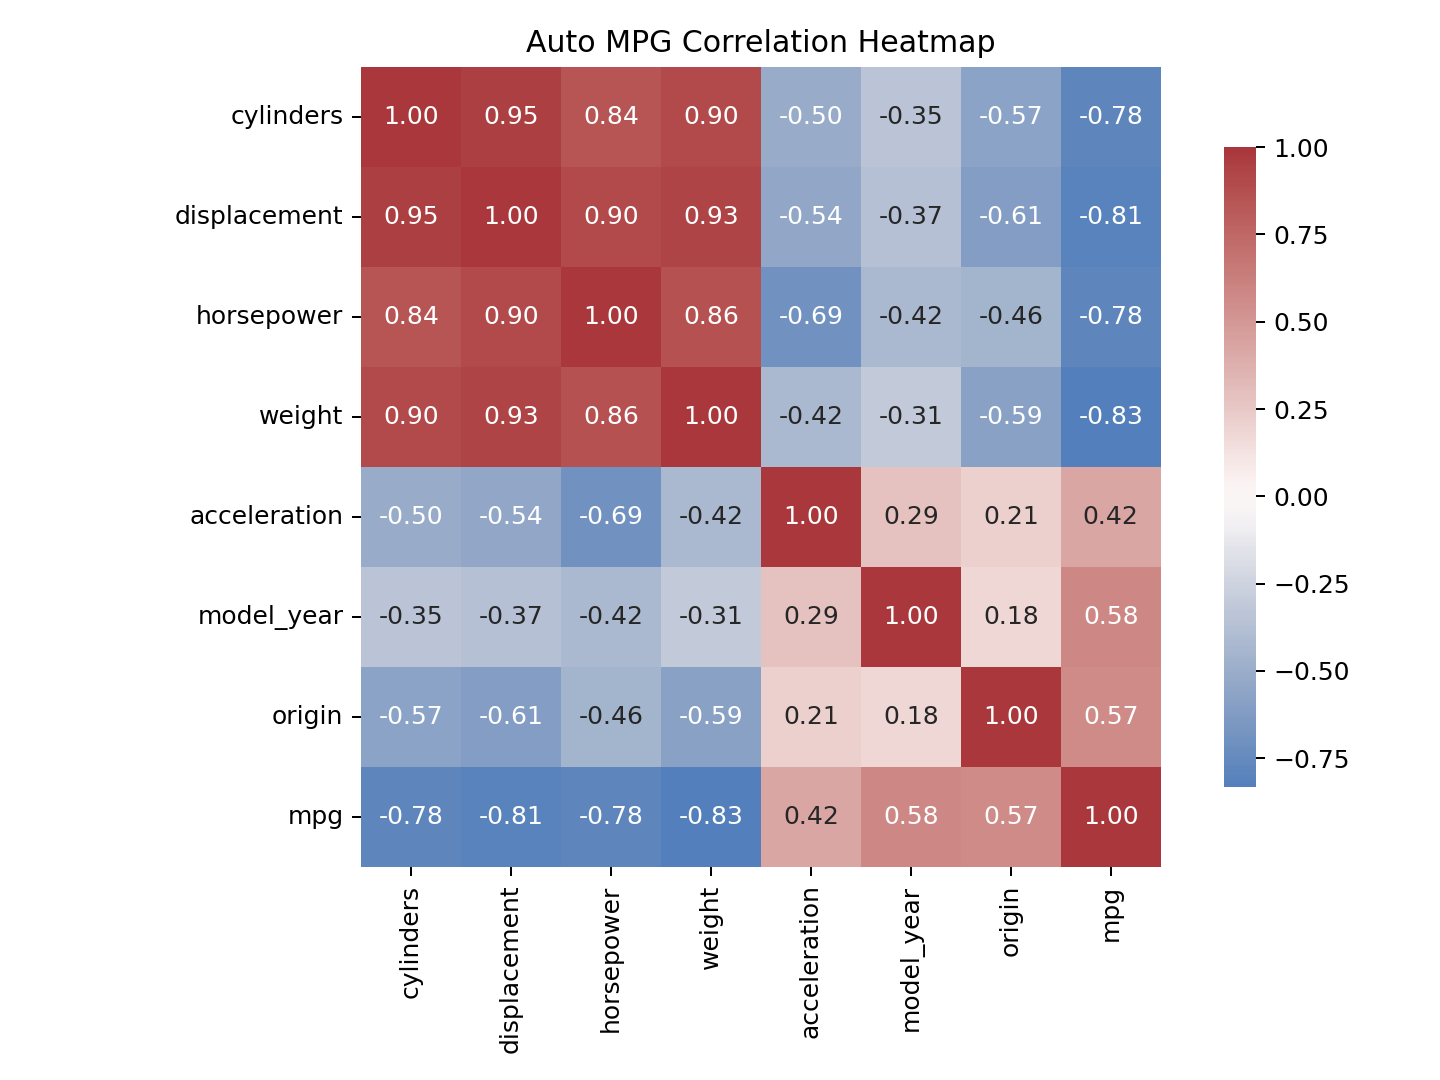
\includegraphics[width=0.65\textwidth]{../results/figures/auto_mpg_heatmap.png}
\caption{Correlation heatmap for Auto MPG.}
\label{fig:auto_mpg_heatmap}
\end{figure}

\begin{table}[H]
\centering
\small
\begin{tabular}{rlr}
\toprule
Rank & Predictor & Absolute correlation \\
\midrule
1 & \textbf{weight} & 0.832244 \\
2 & \textbf{displacement} & 0.805127 \\
3 & horsepower & 0.778427 \\
4 & cylinders & 0.777618 \\
5 & model year & 0.580541 \\
6 & origin & 0.565209 \\
7 & acceleration & 0.423329 \\
\bottomrule
\end{tabular}
\caption{Absolute predictor correlations with \texttt{mpg} for Auto MPG, ranked from strongest to weakest.}
\label{tab:auto_mpg_target_corr}
\end{table}

Table~\ref{tab:auto_mpg_target_corr} lists every predictor's absolute correlation with the target. Absolute correlation measures linear association strength regardless of direction: values closer to 1 indicate stronger linear associations, while values closer to 0 indicate weaker linear associations. The signs of the correlations are shown in the heatmap. The first two predictors, shown in bold, are selected for the separate simple regressions. Weight and displacement have the strongest absolute correlations with MPG. Both correlations are negative: heavier vehicles and larger engine displacement tend to accompany lower MPG in these data. Origin is a categorical code, so its numerical correlation depends on the coding used. These correlations describe associations and do not establish causation.

\begin{table}[H]
\centering
\small
\begin{tabular}{llr}
\toprule
Feature 1 & Feature 2 & Correlation \\
\midrule
cylinders & displacement & 0.950823 \\
displacement & weight & 0.932994 \\
cylinders & weight & 0.897527 \\
displacement & horsepower & 0.897257 \\
horsepower & weight & 0.864538 \\
cylinders & horsepower & 0.842983 \\
\bottomrule
\end{tabular}
\caption{Strongly correlated predictor pairs for Auto MPG ($|r| > 0.75$).}
\label{tab:auto_mpg_predictor_pairs}
\end{table}

Table~\ref{tab:auto_mpg_predictor_pairs} screens predictor pairs using an absolute correlation threshold of 0.75. Each pair appears once, self-correlations and the target are excluded, and the displayed correlations retain their signs. These pairs have strong linear associations and may provide overlapping information if included together in a multiple regression. The simple regressions here use one predictor at a time, so they do not include these pairs jointly.

The two predictors with the largest absolute correlation to the target \texttt{mpg} are \texttt{weight} ($r=-0.8322$) and \texttt{displacement} ($r=-0.8051$).

\subsection{SimpleRegression for the Top Two Predictors}

\paragraph{Predictor: \texttt{weight} (target correlation $r = -0.8322$)}

\textit{ScalaTion \texttt{SimpleRegression} fit report (\texttt{mod.summary()}):}
\begin{verbatim}
    Parameters/Coefficients:
    Var      Estimate    Std. Error 	 t value 	 Pr(>|t|) 	 VIF
----------------------------------------------------------------------------------
    x0	 46.216525	 0.798672	 57.866681	 0.000000	 NA
    x1	 -0.007647	 0.000258	 -29.645082	 0.000000	 1.000000

    Residual standard error: 4.332712 on 390.0 degrees of freedom
    Multiple R-squared:  0.692630,	Adjusted R-squared:  0.691842
    F-statistic: 878.8308864132066 on 1.0 and 390.0 DF,  p-value: -0.0
\end{verbatim}

\textit{Statsmodels \texttt{sm.OLS} fit report (\texttt{model.summary()}):}
\begin{verbatim}
                            OLS Regression Results                            
==============================================================================
Dep. Variable:                    mpg   R-squared:                       0.693
Model:                            OLS   Adj. R-squared:                  0.692
Method:                 Least Squares   F-statistic:                     878.8
Date:                Sun, 06 Sep 2026   Prob (F-statistic):          6.02e-102
Time:                        14:07:39   Log-Likelihood:                -1130.0
No. Observations:                 392   AIC:                             2264.
Df Residuals:                     390   BIC:                             2272.
Df Model:                           1                                         
Covariance Type:            nonrobust                                         
==============================================================================
                 coef    std err          t      P>|t|      [0.025      0.975]
------------------------------------------------------------------------------
const         46.2165      0.799     57.867      0.000      44.646      47.787
weight        -0.0076      0.000    -29.645      0.000      -0.008      -0.007
==============================================================================
Omnibus:                       41.682   Durbin-Watson:                   0.808
Prob(Omnibus):                  0.000   Jarque-Bera (JB):               60.039
Skew:                           0.727   Prob(JB):                     9.18e-14
Kurtosis:                       4.251   Cond. No.                     1.13e+04
==============================================================================

Notes:
[1] Standard Errors assume that the covariance matrix of the errors is correctly specified.
[2] The condition number is large, 1.13e+04. This might indicate that there are
strong multicollinearity or other numerical problems.
\end{verbatim}

\textbf{Summary statement:} $\widehat{\text{mpg}} = 46.2165 - 0.0076 \cdot \text{weight}$, with $R^2 = 0.6926$ (adj.\ $R^2 = 0.6918$), RMSE $= 4.3216$, on $n = 392$ observations. Each 1-unit increase in \texttt{weight} is associated with a $-0.0076$ change in \texttt{mpg}.

\begin{figure}[H]
\centering
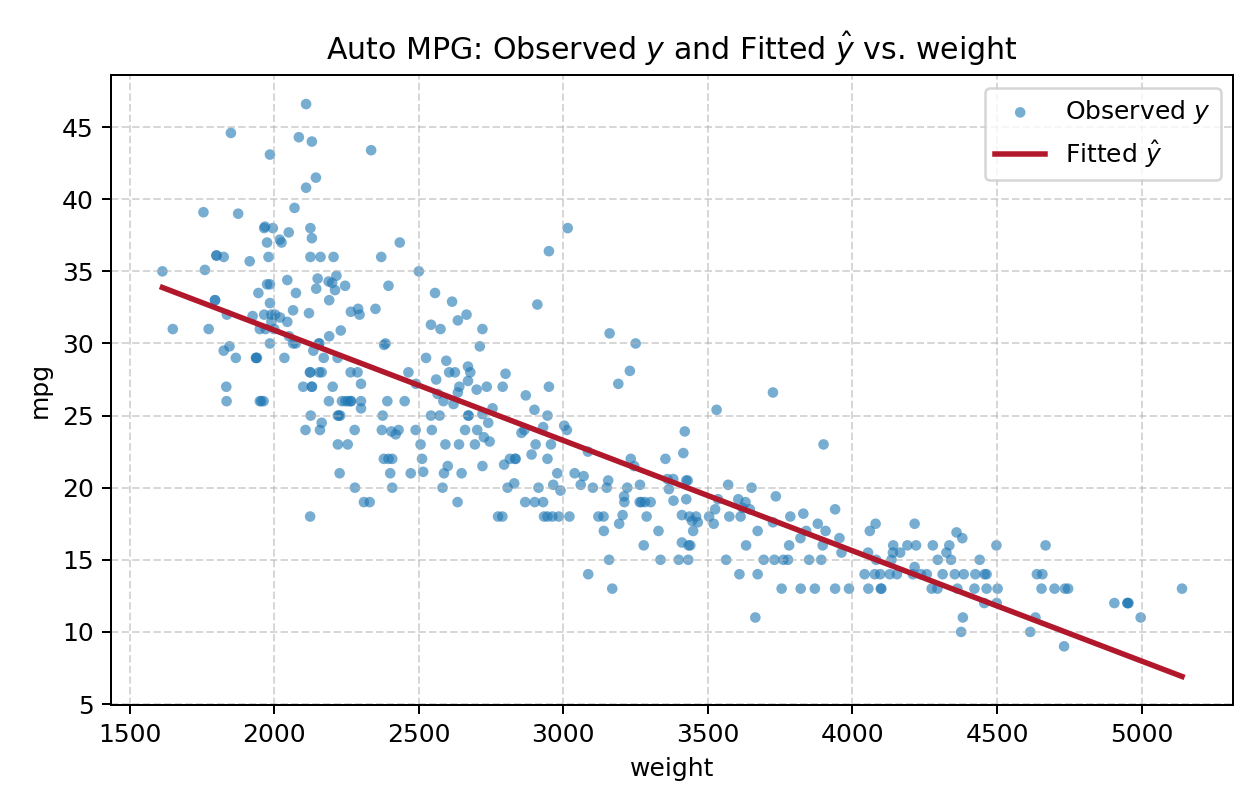
\includegraphics[width=0.7\textwidth]{../results/figures/auto_mpg_weight_regression.png}
\caption{Observed ${y}$ and fitted $\hat{y}$ vs.\ \texttt{weight} for Auto MPG.}
\end{figure}

\paragraph{Predictor: \texttt{displacement} (target correlation $r = -0.8051$)}

\textit{ScalaTion \texttt{SimpleRegression} fit report (\texttt{mod.summary()}):}
\begin{verbatim}
    Parameters/Coefficients:
    Var      Estimate    Std. Error 	 t value 	 Pr(>|t|) 	 VIF
----------------------------------------------------------------------------------
    x0	 35.120636	 0.494428	 71.032840	 0.000000	 NA
    x1	 -0.060051	 0.002240	 -26.808153	 0.000000	 1.000000

    Residual standard error: 4.635101 on 390.0 degrees of freedom
    Multiple R-squared:  0.648229,	Adjusted R-squared:  0.647327
    F-statistic: 718.6770763503415 on 1.0 and 390.0 DF,  p-value: -0.0
\end{verbatim}

\textit{Statsmodels \texttt{sm.OLS} fit report (\texttt{model.summary()}):}
\begin{verbatim}
                            OLS Regression Results                            
==============================================================================
Dep. Variable:                    mpg   R-squared:                       0.648
Model:                            OLS   Adj. R-squared:                  0.647
Method:                 Least Squares   F-statistic:                     718.7
Date:                Sun, 06 Sep 2026   Prob (F-statistic):           1.66e-90
Time:                        14:07:39   Log-Likelihood:                -1156.4
No. Observations:                 392   AIC:                             2317.
Df Residuals:                     390   BIC:                             2325.
Df Model:                           1                                         
Covariance Type:            nonrobust                                         
================================================================================
                   coef    std err          t      P>|t|      [0.025      0.975]
--------------------------------------------------------------------------------
const           35.1206      0.494     71.033      0.000      34.149      36.093
displacement    -0.0601      0.002    -26.808      0.000      -0.064      -0.056
==============================================================================
Omnibus:                       41.308   Durbin-Watson:                   0.926
Prob(Omnibus):                  0.000   Jarque-Bera (JB):               61.139
Skew:                           0.709   Prob(JB):                     5.30e-14
Kurtosis:                       4.317   Cond. No.                         466.
==============================================================================

Notes:
[1] Standard Errors assume that the covariance matrix of the errors is correctly specified.
\end{verbatim}

\textbf{Summary statement:} $\widehat{\text{mpg}} = 35.1206 - 0.0601 \cdot \text{displacement}$, with $R^2 = 0.6482$ (adj.\ $R^2 = 0.6473$), RMSE $= 4.6233$, on $n = 392$ observations. Each 1-unit increase in \texttt{displacement} is associated with a $-0.0601$ change in \texttt{mpg}.

\begin{figure}[H]
\centering
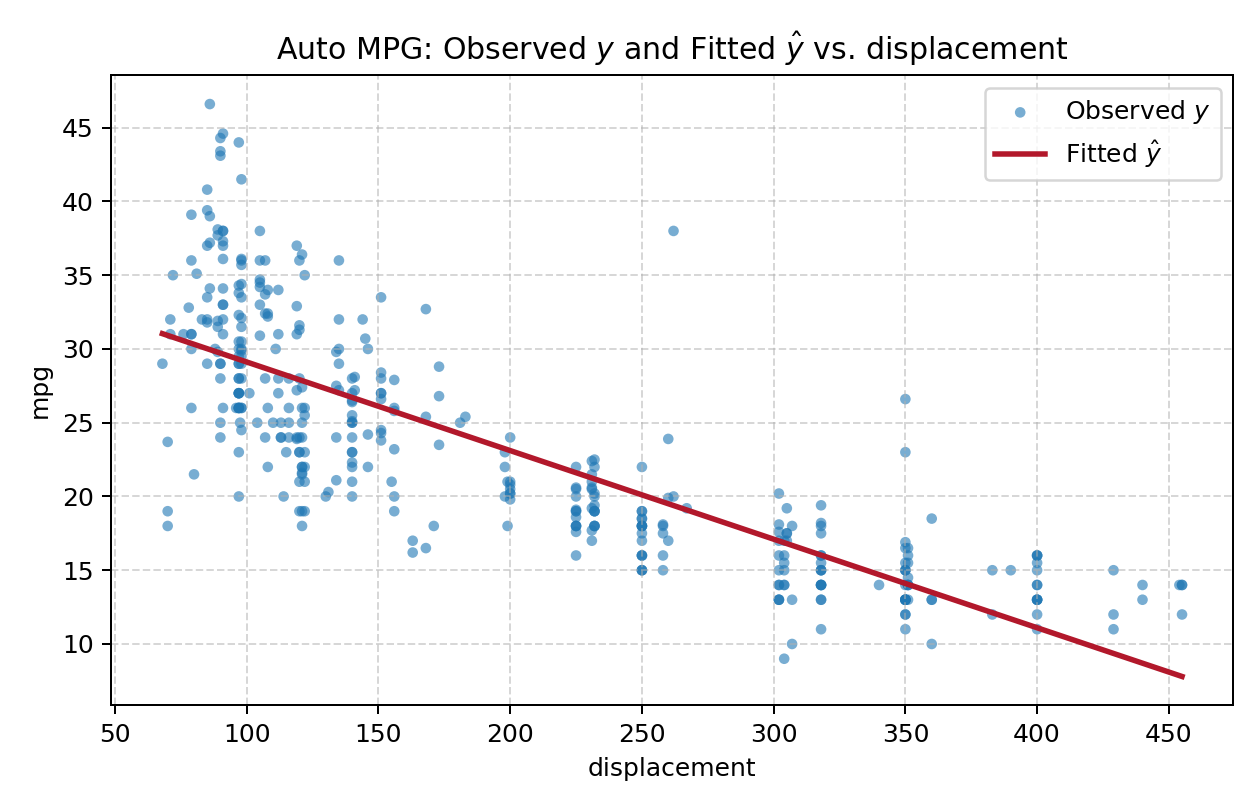
\includegraphics[width=0.7\textwidth]{../results/figures/auto_mpg_displacement_regression.png}
\caption{Observed ${y}$ and fitted $\hat{y}$ vs.\ \texttt{displacement} for Auto MPG.}
\end{figure}


\subsection{Discussion}
Both top predictors, vehicle weight and engine displacement, show strong negative linear association with fuel economy, consistent with basic automotive thermodynamics: heavier vehicles and larger engines consume more fuel per mile. The observed-vs-fitted scatter plots show visible curvature -- mpg falls steeply at low weight and levels off at high weight. The visible curvature suggests that reciprocal or polynomial models may improve fit.


\section{Concrete Compressive Strength Dataset}

\subsection{Preprocessing: String Values, Missing Values, and Outliers}
\begin{itemize}
    \item \textbf{String Values:} The dataset contains seven ingredient quantities measured in kg/m$^3$, curing age in days, and compressive strength in MPa; the only text encountered was the original Excel header row, which was renamed to clean snake\_case identifiers. No categorical/string encoding was required.
    \item \textbf{Missing Values:} Zero missing values across all 1{,}030 mixture observations; no imputation or row deletion was necessary.
    \item \textbf{Outliers:} Tukey's IQR rule flags 59 instances in \texttt{age} (mixes cured up to 365 days), 10 in \texttt{superplasticizer}, 9 in \texttt{water}, 5 in \texttt{fine\_aggregate}, 2 in \texttt{blast\_furnace\_slag}, and 4 in the target \texttt{compressive\_strength\_mpa}. These reflect legitimate specialized high-strength mix designs and extended curing trials and were retained.
\end{itemize}

\subsection{Statistical Summaries for Each Feature/Variable}
\begin{table}[H]
\centering
\small
\begin{tabular}{lrrrrrrrrr}
\toprule
Variable & mean & std & min & 25\% & 50\% & 75\% & max & missing & outliers \\
\midrule
cement & 281.1656 & 104.5071 & 102.0000 & 192.3750 & 272.9000 & 350.0000 & 540.0000 & 0 & 0 \\
blast\_furnace\_slag & 73.8955 & 86.2791 & 0.0000 & 0.0000 & 22.0000 & 142.9500 & 359.4000 & 0 & 2 \\
fly\_ash & 54.1871 & 63.9965 & 0.0000 & 0.0000 & 0.0000 & 118.2700 & 200.1000 & 0 & 0 \\
water & 181.5664 & 21.3556 & 121.7500 & 164.9000 & 185.0000 & 192.0000 & 247.0000 & 0 & 9 \\
superplasticizer & 6.2031 & 5.9735 & 0.0000 & 0.0000 & 6.3500 & 10.1600 & 32.2000 & 0 & 10 \\
coarse\_aggregate & 972.9186 & 77.7538 & 801.0000 & 932.0000 & 968.0000 & 1029.4000 & 1145.0000 & 0 & 0 \\
fine\_aggregate & 773.5789 & 80.1754 & 594.0000 & 730.9500 & 779.5100 & 824.0000 & 992.6000 & 0 & 5 \\
age & 45.6621 & 63.1699 & 1.0000 & 7.0000 & 28.0000 & 56.0000 & 365.0000 & 0 & 59 \\
compressive\_strength\_mpa & 35.8178 & 16.7057 & 2.3318 & 23.7071 & 34.4428 & 46.1363 & 82.5992 & 0 & 4 \\
\bottomrule
\end{tabular}
\caption{Descriptive statistics for Concrete Compressive Strength ($n=1030$, $p=9$ columns).}
\end{table}

\subsection{Correlation Analysis: Matrix and HeatMap}
The full Pearson correlation matrix is printed by \texttt{xy.corr} in ScalaTion and \texttt{df.corr()} in Statsmodels/pandas; both agree exactly. Figure~\ref{fig:concrete_heatmap} shows the heatmap (rendered via Statsmodels/seaborn; ScalaTion's \texttt{HeatMap} class from \texttt{scalation.mathstat} displays the identical matrix in an interactive window via \texttt{project1HeatMaps}).

\begin{figure}[H]
\centering
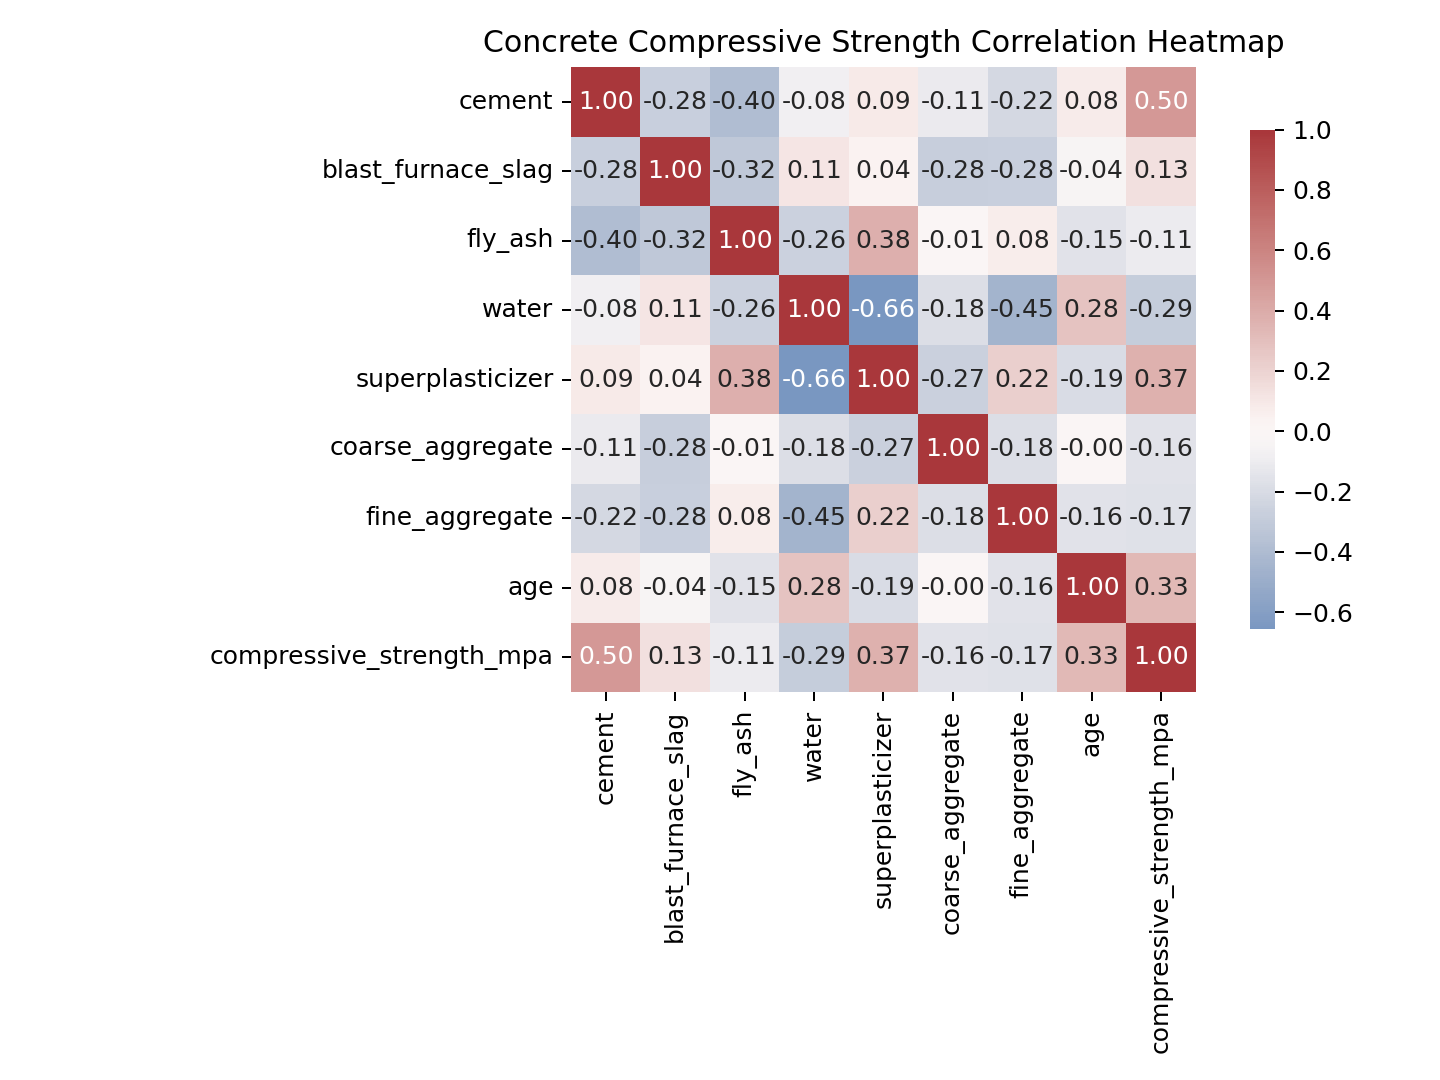
\includegraphics[width=0.65\textwidth]{../results/figures/concrete_heatmap.png}
\caption{Correlation heatmap for Concrete Compressive Strength.}
\label{fig:concrete_heatmap}
\end{figure}

\begin{table}[H]
\centering
\small
\begin{tabular}{rlr}
\toprule
Rank & Predictor & Absolute correlation \\
\midrule
1 & \textbf{cement} & 0.497833 \\
2 & \textbf{superplasticizer} & 0.366102 \\
3 & age & 0.328877 \\
4 & water & 0.289613 \\
5 & fine aggregate & 0.167249 \\
6 & coarse aggregate & 0.164928 \\
7 & blast furnace slag & 0.134824 \\
8 & fly ash & 0.105753 \\
\bottomrule
\end{tabular}
\caption{Absolute predictor correlations with \texttt{compressive\_strength\_mpa} for Concrete Compressive Strength, ranked from strongest to weakest.}
\label{tab:concrete_target_corr}
\end{table}

Table~\ref{tab:concrete_target_corr} lists every predictor's absolute correlation with the target. Absolute correlation measures linear association strength regardless of direction: values closer to 1 indicate stronger linear associations, while values closer to 0 indicate weaker linear associations. The signs of the correlations are shown in the heatmap. The first two predictors, shown in bold, are selected for the separate simple regressions. Cement and superplasticizer have the strongest absolute correlations with compressive strength. Both correlations are positive: higher quantities are associated with higher strength in these separate pairwise comparisons. These correlations describe associations and do not establish causation.

\begin{table}[H]
\centering
\small
\begin{tabular}{llr}
\toprule
Feature 1 & Feature 2 & Correlation \\
\midrule
\multicolumn{3}{c}{No predictor pairs have $|r| > 0.75$.} \\
\bottomrule
\end{tabular}
\caption{Strongly correlated predictor pairs for Concrete Compressive Strength ($|r| > 0.75$).}
\label{tab:concrete_predictor_pairs}
\end{table}

Table~\ref{tab:concrete_predictor_pairs} screens predictor pairs using an absolute correlation threshold of 0.75. Each pair appears once, self-correlations and the target are excluded, and the displayed correlations retain their signs. No predictor pair exceeds this screening threshold. This does not rule out multicollinearity involving combinations of several predictors in a future multiple regression.

The two predictors with the largest absolute correlation to the target \texttt{compressive\_strength\_mpa} are \texttt{cement} ($r=0.4978$) and \texttt{superplasticizer} ($r=0.3661$).

\subsection{SimpleRegression for the Top Two Predictors}

\paragraph{Predictor: \texttt{cement} (target correlation $r = 0.4978$)}

\textit{ScalaTion \texttt{SimpleRegression} fit report (\texttt{mod.summary()}):}
\begin{verbatim}
    Parameters/Coefficients:
    Var      Estimate    Std. Error 	 t value 	 Pr(>|t|) 	 VIF
----------------------------------------------------------------------------------
    x0	 13.442795	 1.296925	 10.365129	 0.000000	 NA
    x1	 0.079580	 0.004324	 18.404505	 0.000000	 1.000000

    Residual standard error: 14.495431 on 1028.0 degrees of freedom
    Multiple R-squared:  0.247837,	Adjusted R-squared:  0.247106
    F-statistic: 338.7257936916475 on 1.0 and 1028.0 DF,  p-value: -0.0
\end{verbatim}

\textit{Statsmodels \texttt{sm.OLS} fit report (\texttt{model.summary()}):}
\begin{verbatim}
                               OLS Regression Results                               
====================================================================================
Dep. Variable:     compressive_strength_mpa   R-squared:                       0.248
Model:                                  OLS   Adj. R-squared:                  0.247
Method:                       Least Squares   F-statistic:                     338.7
Date:                      Sun, 06 Sep 2026   Prob (F-statistic):           1.32e-65
Time:                              14:07:39   Log-Likelihood:                -4214.6
No. Observations:                      1030   AIC:                             8433.
Df Residuals:                          1028   BIC:                             8443.
Df Model:                                 1                                         
Covariance Type:                  nonrobust                                         
==============================================================================
                 coef    std err          t      P>|t|      [0.025      0.975]
------------------------------------------------------------------------------
const         13.4428      1.297     10.365      0.000      10.898      15.988
cement         0.0796      0.004     18.405      0.000       0.071       0.088
==============================================================================
Omnibus:                       19.695   Durbin-Watson:                   1.012
Prob(Omnibus):                  0.000   Jarque-Bera (JB):               17.890
Skew:                           0.271   Prob(JB):                     0.000130
Kurtosis:                       2.649   Cond. No.                         861.
==============================================================================

Notes:
[1] Standard Errors assume that the covariance matrix of the errors is correctly specified.
\end{verbatim}

\textbf{Summary statement:} $\widehat{\text{compressive\_strength\_mpa}} = 13.4428 + 0.0796 \cdot \text{cement}$, with $R^2 = 0.2478$ (adj.\ $R^2 = 0.2471$), RMSE $= 14.4814$, on $n = 1030$ observations. Each 1-unit increase in \texttt{cement} is associated with a $0.0796$ change in \texttt{compressive\_strength\_mpa}.

\begin{figure}[H]
\centering
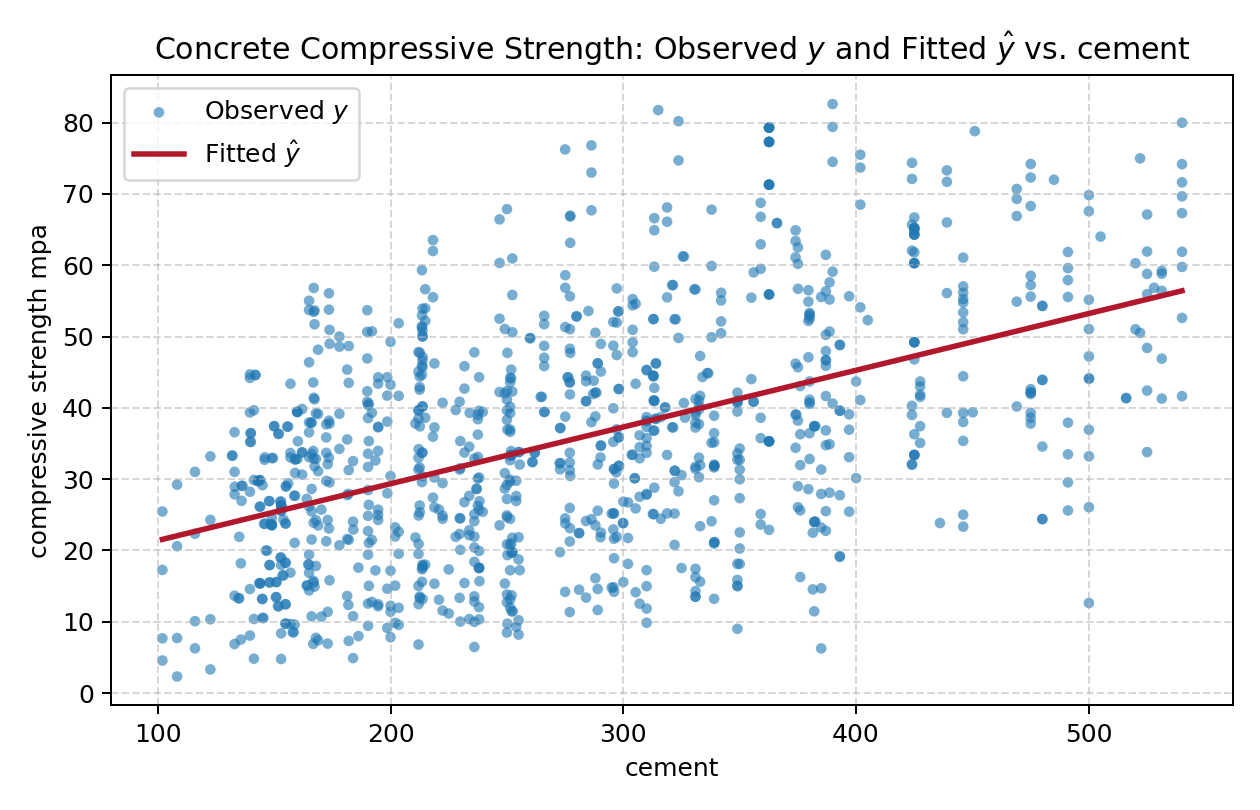
\includegraphics[width=0.7\textwidth]{../results/figures/concrete_cement_regression.png}
\caption{Observed ${y}$ and fitted $\hat{y}$ vs.\ \texttt{cement} for Concrete Compressive Strength.}
\end{figure}

\paragraph{Predictor: \texttt{superplasticizer} (target correlation $r = 0.3661$)}

\textit{ScalaTion \texttt{SimpleRegression} fit report (\texttt{mod.summary()}):}
\begin{verbatim}
    Parameters/Coefficients:
    Var      Estimate    Std. Error 	 t value 	 Pr(>|t|) 	 VIF
----------------------------------------------------------------------------------
    x0	 29.466751	 0.698839	 42.165264	 0.000000	 NA
    x1	 1.023855	 0.081169	 12.613854	 0.000000	 1.000000

    Residual standard error: 15.553440 on 1028.0 degrees of freedom
    Multiple R-squared:  0.134031,	Adjusted R-squared:  0.133189
    F-statistic: 159.1093217311018 on 1.0 and 1028.0 DF,  p-value: -0.0
\end{verbatim}

\textit{Statsmodels \texttt{sm.OLS} fit report (\texttt{model.summary()}):}
\begin{verbatim}
                               OLS Regression Results                               
====================================================================================
Dep. Variable:     compressive_strength_mpa   R-squared:                       0.134
Model:                                  OLS   Adj. R-squared:                  0.133
Method:                       Least Squares   F-statistic:                     159.1
Date:                      Sun, 06 Sep 2026   Prob (F-statistic):           5.08e-34
Time:                              14:07:39   Log-Likelihood:                -4287.1
No. Observations:                      1030   AIC:                             8578.
Df Residuals:                          1028   BIC:                             8588.
Df Model:                                 1                                         
Covariance Type:                  nonrobust                                         
====================================================================================
                       coef    std err          t      P>|t|      [0.025      0.975]
------------------------------------------------------------------------------------
const               29.4668      0.699     42.165      0.000      28.095      30.838
superplasticizer     1.0239      0.081     12.614      0.000       0.865       1.183
==============================================================================
Omnibus:                       24.083   Durbin-Watson:                   1.052
Prob(Omnibus):                  0.000   Jarque-Bera (JB):               24.387
Skew:                           0.353   Prob(JB):                     5.06e-06
Kurtosis:                       2.738   Cond. No.                         12.5
==============================================================================

Notes:
[1] Standard Errors assume that the covariance matrix of the errors is correctly specified.
\end{verbatim}

\textbf{Summary statement:} $\widehat{\text{compressive\_strength\_mpa}} = 29.4668 + 1.0239 \cdot \text{superplasticizer}$, with $R^2 = 0.1340$ (adj.\ $R^2 = 0.1332$), RMSE $= 15.5383$, on $n = 1030$ observations. Each 1-unit increase in \texttt{superplasticizer} is associated with a $1.0239$ change in \texttt{compressive\_strength\_mpa}.

\begin{figure}[H]
\centering
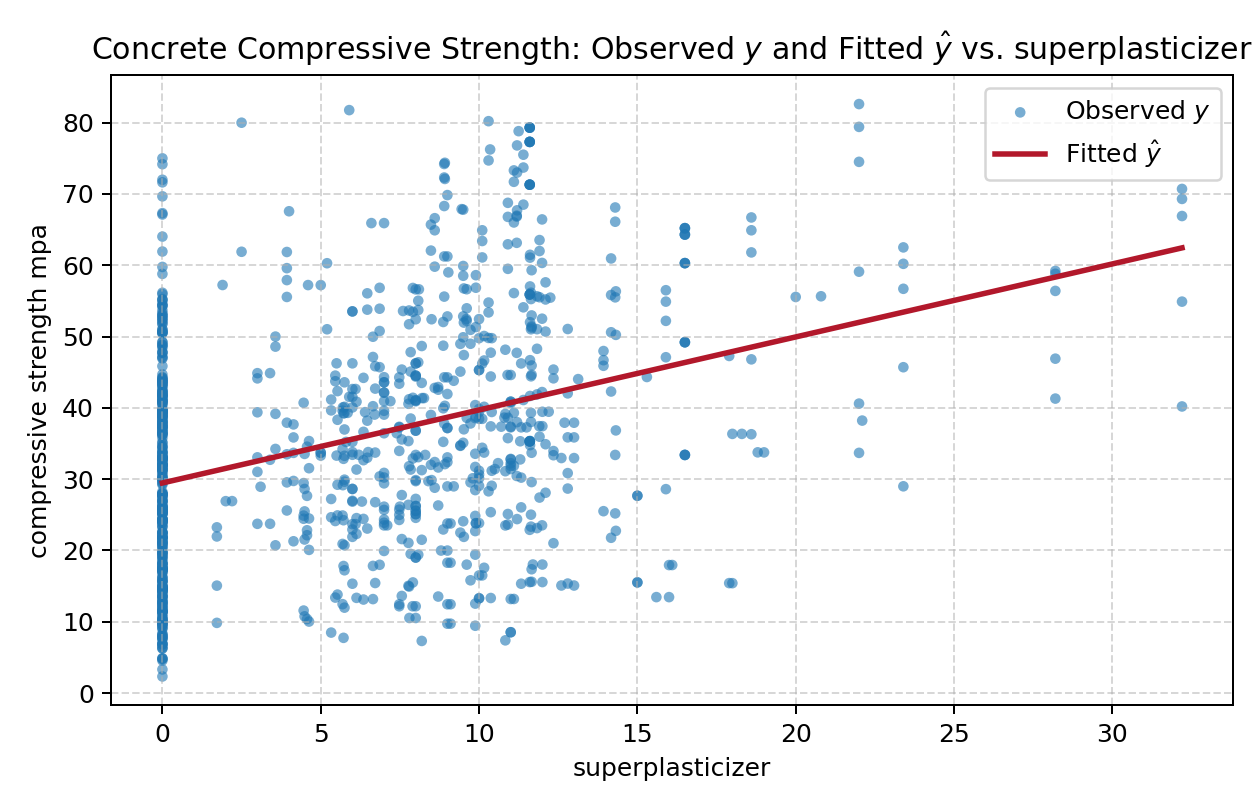
\includegraphics[width=0.7\textwidth]{../results/figures/concrete_superplasticizer_regression.png}
\caption{Observed ${y}$ and fitted $\hat{y}$ vs.\ \texttt{superplasticizer} for Concrete Compressive Strength.}
\end{figure}


\subsection{Discussion}
Cement content ($R^2=0.248$) is the strongest single predictor of compressive strength, consistent with its role as the primary binding agent in the hydration reaction; superplasticizer ($R^2=0.134$) improves strength by reducing the water needed to maintain workability, which densifies the cement matrix. However, over 75\% of strength variance is left unexplained by either predictor alone, which motivates multiple regression incorporating water-to-cement ratio and curing age.


\section{Airfoil Self-Noise Dataset}

\subsection{Preprocessing: String Values, Missing Values, and Outliers}
\begin{itemize}
    \item \textbf{String Values:} The source \texttt{.dat} file is whitespace-delimited numeric data with no header and no text columns; descriptive engineering names with SI units (Hz, degrees, m, m/s, dB) were assigned during CSV conversion. No string decoding was needed.
    \item \textbf{Missing Values:} Zero missing observations across all 1{,}503 NASA wind-tunnel test runs; no rows were dropped.
    \item \textbf{Outliers:} Tukey's 1.5$\times$IQR rule flags 86 outliers in \texttt{frequency\_hz} (tests extend up to 20{,}000~Hz), 30 in \texttt{angle\_attack\_deg} (up to 22.2$^\circ$, near stall), 124 in \texttt{suction\_displacement\_thickness\_m}, and 4 in the target \texttt{scaled\_sound\_pressure\_db}. All reflect genuine aerodynamic/boundary-layer phenomena from controlled wind-tunnel testing and were retained.
\end{itemize}

\subsection{Statistical Summaries for Each Feature/Variable}
\begin{table}[H]
\centering
\resizebox{\textwidth}{!}{%
\begin{tabular}{lrrrrrrrrr}
\toprule
Variable & mean & std & min & 25\% & 50\% & 75\% & max & missing & outliers \\
\midrule
frequency\_hz & 2886.3806 & 3152.5731 & 200.0000 & 800.0000 & 1600.0000 & 4000.0000 & 20000.0000 & 0 & 86 \\
angle\_attack\_deg & 6.7823 & 5.9181 & 0.0000 & 2.0000 & 5.4000 & 9.9000 & 22.2000 & 0 & 30 \\
chord\_length\_m & 0.1365 & 0.0935 & 0.0254 & 0.0508 & 0.1016 & 0.2286 & 0.3048 & 0 & 0 \\
free\_stream\_velocity\_ms & 50.8607 & 15.5728 & 31.7000 & 39.6000 & 39.6000 & 71.3000 & 71.3000 & 0 & 0 \\
suction\_displacement\_thickness\_m & 0.0111 & 0.0132 & 0.0004 & 0.0025 & 0.0050 & 0.0156 & 0.0584 & 0 & 124 \\
scaled\_sound\_pressure\_db & 124.8359 & 6.8987 & 103.3800 & 120.1910 & 125.7210 & 129.9955 & 140.9870 & 0 & 4 \\
\bottomrule
\end{tabular}%
}
\caption{Descriptive statistics for Airfoil Self-Noise ($n=1503$, $p=6$ columns).}
\end{table}

\subsection{Correlation Analysis: Matrix and HeatMap}
The full Pearson correlation matrix is printed by \texttt{xy.corr} in ScalaTion and \texttt{df.corr()} in Statsmodels/pandas; both agree exactly. Figure~\ref{fig:airfoil_heatmap} shows the heatmap (rendered via Statsmodels/seaborn; ScalaTion's \texttt{HeatMap} class from \texttt{scalation.mathstat} displays the identical matrix in an interactive window via \texttt{project1HeatMaps}).

\begin{figure}[H]
\centering
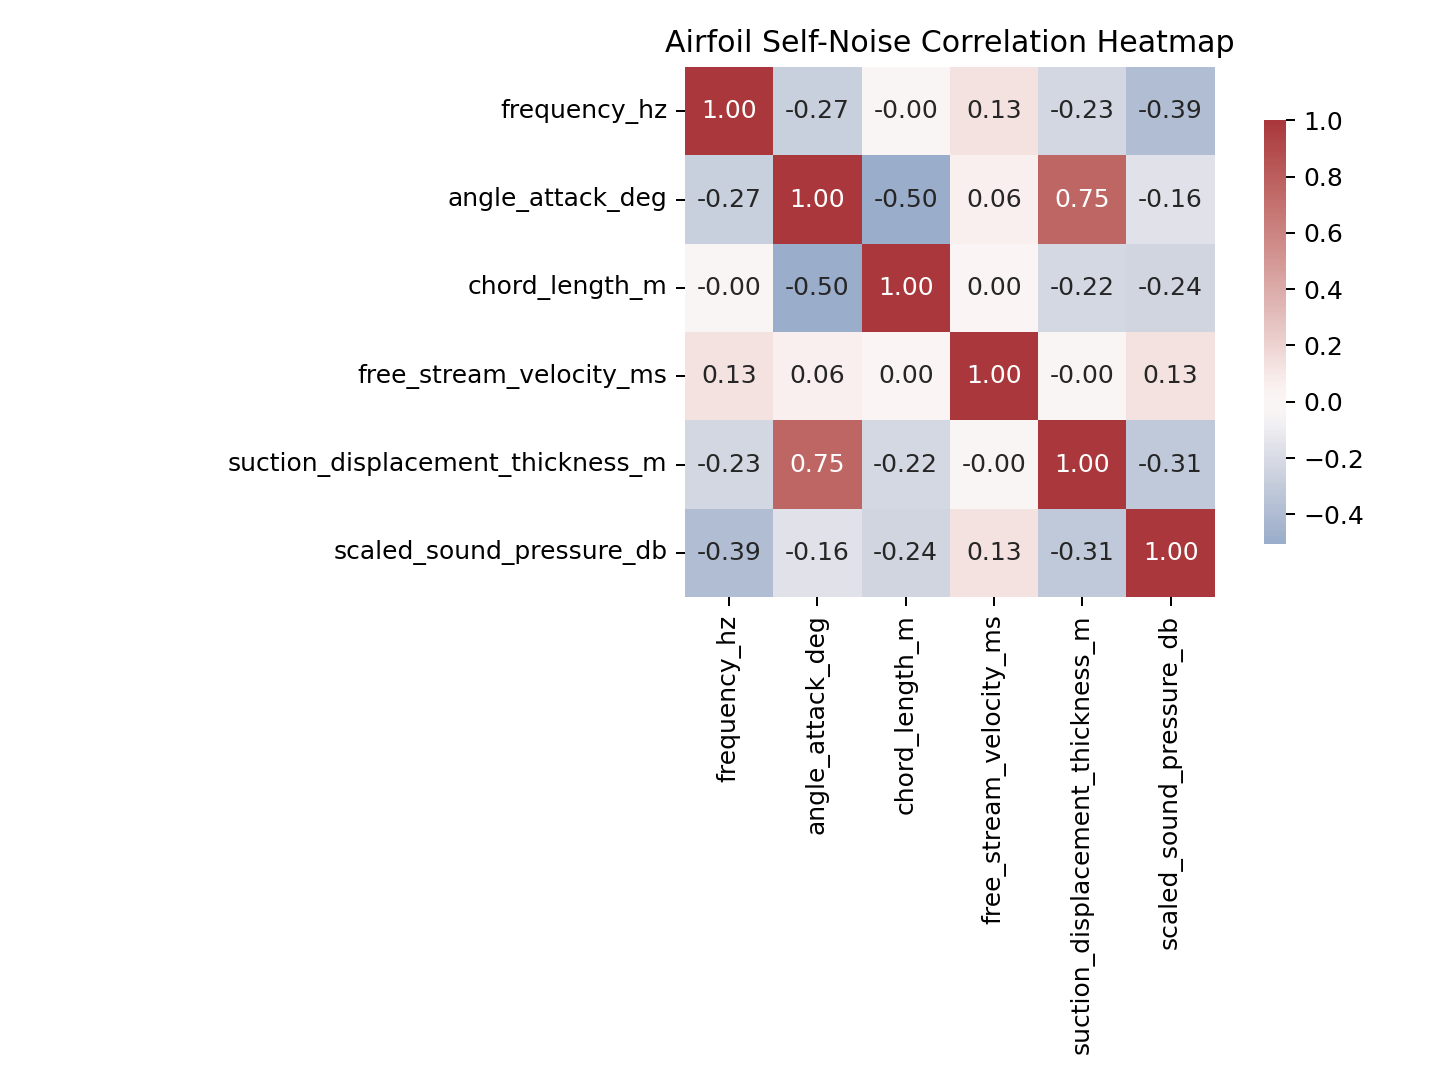
\includegraphics[width=0.65\textwidth]{../results/figures/airfoil_heatmap.png}
\caption{Correlation heatmap for Airfoil Self-Noise.}
\label{fig:airfoil_heatmap}
\end{figure}

\begin{table}[H]
\centering
\small
\begin{tabular}{rlr}
\toprule
Rank & Predictor & Absolute correlation \\
\midrule
1 & \textbf{frequency hz} & 0.390711 \\
2 & \textbf{suction displacement thickness m} & 0.312670 \\
3 & chord length m & 0.236162 \\
4 & angle attack deg & 0.156108 \\
5 & free stream velocity ms & 0.125103 \\
\bottomrule
\end{tabular}
\caption{Absolute predictor correlations with \texttt{scaled\_sound\_pressure\_db} for Airfoil Self-Noise, ranked from strongest to weakest.}
\label{tab:airfoil_target_corr}
\end{table}

Table~\ref{tab:airfoil_target_corr} lists every predictor's absolute correlation with the target. Absolute correlation measures linear association strength regardless of direction: values closer to 1 indicate stronger linear associations, while values closer to 0 indicate weaker linear associations. The signs of the correlations are shown in the heatmap. The first two predictors, shown in bold, are selected for the separate simple regressions. Frequency and suction-side displacement thickness have the strongest absolute correlations with scaled sound pressure level. Both correlations are negative, indicating that larger values tend to accompany lower sound pressure levels in these data. These correlations describe associations and do not establish causation.

\begin{table}[H]
\centering
\small
\begin{tabular}{llr}
\toprule
Feature 1 & Feature 2 & Correlation \\
\midrule
angle attack deg & suction displacement thickness m & 0.753394 \\
\bottomrule
\end{tabular}
\caption{Strongly correlated predictor pairs for Airfoil Self-Noise ($|r| > 0.75$).}
\label{tab:airfoil_predictor_pairs}
\end{table}

Table~\ref{tab:airfoil_predictor_pairs} screens predictor pairs using an absolute correlation threshold of 0.75. Each pair appears once, self-correlations and the target are excluded, and the displayed correlations retain their signs. These pairs have strong linear associations and may provide overlapping information if included together in a multiple regression. The simple regressions here use one predictor at a time, so they do not include these pairs jointly.

The two predictors with the largest absolute correlation to the target \texttt{scaled\_sound\_pressure\_db} are \texttt{frequency\_hz} ($r=-0.3907$) and \texttt{suction\_displacement\_thickness\_m} ($r=-0.3127$).

\subsection{SimpleRegression for the Top Two Predictors}

\paragraph{Predictor: \texttt{frequency\_hz} (target correlation $r = -0.3907$)}

\textit{ScalaTion \texttt{SimpleRegression} fit report (\texttt{mod.summary()}):}
\begin{verbatim}
    Parameters/Coefficients:
    Var      Estimate    Std. Error 	 t value 	 Pr(>|t|) 	 VIF
----------------------------------------------------------------------------------
    x0	 127.303738	 0.222192	 572.944445	 0.000000	 NA
    x1	 -0.000855	 0.000052	 -16.444339	 0.000000	 1.000000

    Residual standard error: 6.352420 on 1501.0 degrees of freedom
    Multiple R-squared:  0.152655,	Adjusted R-squared:  0.152091
    F-statistic: 270.4162724626191 on 1.0 and 1501.0 DF,  p-value: -0.0
\end{verbatim}

\textit{Statsmodels \texttt{sm.OLS} fit report (\texttt{model.summary()}):}
\begin{verbatim}
                               OLS Regression Results                               
====================================================================================
Dep. Variable:     scaled_sound_pressure_db   R-squared:                       0.153
Model:                                  OLS   Adj. R-squared:                  0.152
Method:                       Least Squares   F-statistic:                     270.4
Date:                      Sun, 06 Sep 2026   Prob (F-statistic):           5.36e-56
Time:                              14:07:39   Log-Likelihood:                -4910.5
No. Observations:                      1503   AIC:                             9825.
Df Residuals:                          1501   BIC:                             9836.
Df Model:                                 1                                         
Covariance Type:                  nonrobust                                         
================================================================================
                   coef    std err          t      P>|t|      [0.025      0.975]
--------------------------------------------------------------------------------
const          127.3037      0.222    572.944      0.000     126.868     127.740
frequency_hz    -0.0009    5.2e-05    -16.444      0.000      -0.001      -0.001
==============================================================================
Omnibus:                        4.973   Durbin-Watson:                   0.255
Prob(Omnibus):                  0.083   Jarque-Bera (JB):                5.002
Skew:                          -0.126   Prob(JB):                       0.0820
Kurtosis:                       2.873   Cond. No.                     5.80e+03
==============================================================================

Notes:
[1] Standard Errors assume that the covariance matrix of the errors is correctly specified.
[2] The condition number is large, 5.8e+03. This might indicate that there are
strong multicollinearity or other numerical problems.
\end{verbatim}

\textbf{Summary statement:} $\widehat{\text{scaled\_sound\_pressure\_db}} = 127.3037 - 0.000854979 \cdot \text{frequency\_hz}$, with $R^2 = 0.1527$ (adj.\ $R^2 = 0.1521$), RMSE $= 6.3482$, on $n = 1503$ observations. Each 1-unit increase in \texttt{frequency\_hz} is associated with a $-0.000854979$ change in \texttt{scaled\_sound\_pressure\_db}.

\begin{figure}[H]
\centering
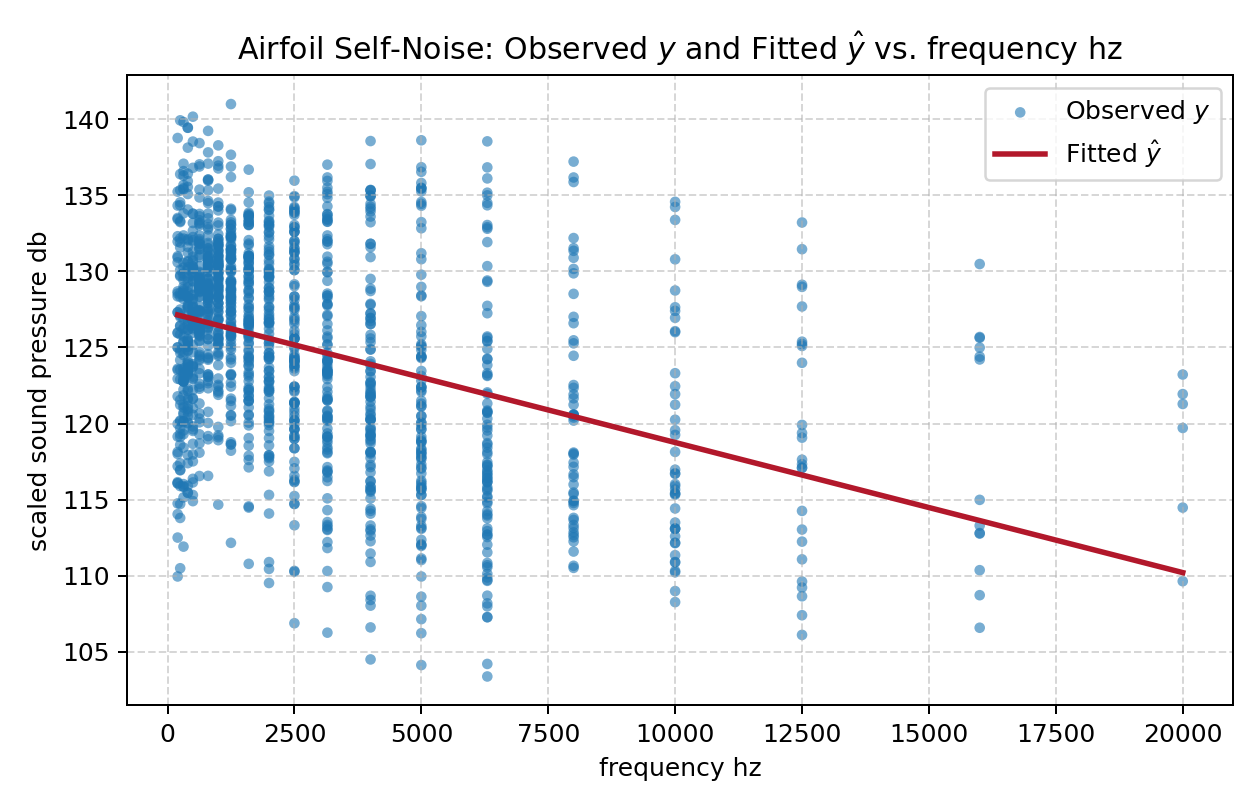
\includegraphics[width=0.7\textwidth]{../results/figures/airfoil_frequency_hz_regression.png}
\caption{Observed ${y}$ and fitted $\hat{y}$ vs.\ \texttt{frequency\_hz} for Airfoil Self-Noise.}
\end{figure}

\paragraph{Predictor: \texttt{suction\_displacement\_thickness\_m} (target correlation $r = -0.3127$)}

\textit{ScalaTion \texttt{SimpleRegression} fit report (\texttt{mod.summary()}):}
\begin{verbatim}
    Parameters/Coefficients:
    Var      Estimate    Std. Error 	 t value 	 Pr(>|t|) 	 VIF
----------------------------------------------------------------------------------
    x0	 126.663189	 0.221623	 571.526554	 0.000000	 NA
    x1	 -164.027463	 12.861784	 -12.753088	 0.000000	 1.000000

    Residual standard error: 6.554954 on 1501.0 degrees of freedom
    Multiple R-squared:  0.097762,	Adjusted R-squared:  0.097161
    F-statistic: 162.64126345742537 on 1.0 and 1501.0 DF,  p-value: -0.0
\end{verbatim}

\textit{Statsmodels \texttt{sm.OLS} fit report (\texttt{model.summary()}):}
\begin{verbatim}
                               OLS Regression Results                               
====================================================================================
Dep. Variable:     scaled_sound_pressure_db   R-squared:                       0.098
Model:                                  OLS   Adj. R-squared:                  0.097
Method:                       Least Squares   F-statistic:                     162.6
Date:                      Sun, 06 Sep 2026   Prob (F-statistic):           1.92e-35
Time:                              14:07:39   Log-Likelihood:                -4957.6
No. Observations:                      1503   AIC:                             9919.
Df Residuals:                          1501   BIC:                             9930.
Df Model:                                 1                                         
Covariance Type:                  nonrobust                                         
====================================================================================================
                                       coef    std err          t      P>|t|      [0.025      0.975]
----------------------------------------------------------------------------------------------------
const                              126.6632      0.222    571.527      0.000     126.228     127.098
suction_displacement_thickness_m  -164.0275     12.862    -12.753      0.000    -189.256    -138.798
==============================================================================
Omnibus:                       26.870   Durbin-Watson:                   0.364
Prob(Omnibus):                  0.000   Jarque-Bera (JB):               25.468
Skew:                          -0.280   Prob(JB):                     2.95e-06
Kurtosis:                       2.694   Cond. No.                         76.1
==============================================================================

Notes:
[1] Standard Errors assume that the covariance matrix of the errors is correctly specified.
\end{verbatim}

\textbf{Summary statement:} $\widehat{\text{scaled\_sound\_pressure\_db}} = 126.6632 - 164.0275 \cdot \text{suction\_displacement\_thickness\_m}$, with $R^2 = 0.0978$ (adj.\ $R^2 = 0.0972$), RMSE $= 6.5506$, on $n = 1503$ observations. Each 1-unit increase in \texttt{suction\_displacement\_thickness\_m} is associated with a $-164.0275$ change in \texttt{scaled\_sound\_pressure\_db}.

\begin{figure}[H]
\centering
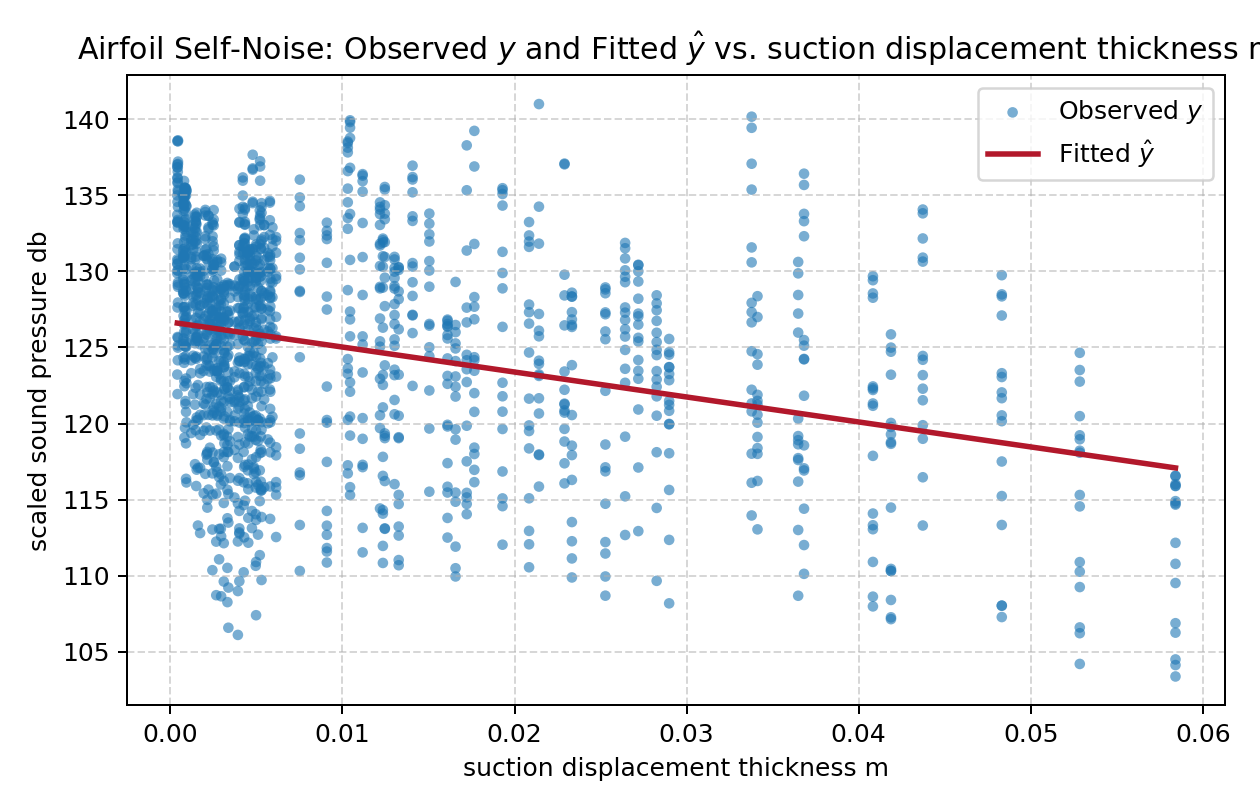
\includegraphics[width=0.7\textwidth]{../results/figures/airfoil_suction_displacement_thickness_m_regression.png}
\caption{Observed ${y}$ and fitted $\hat{y}$ vs.\ \texttt{suction\_displacement\_thickness\_m} for Airfoil Self-Noise.}
\end{figure}


\subsection{Discussion}
Frequency and suction-side displacement thickness are negatively associated with sound pressure level. Their separate linear models explain approximately 15.3\% and 9.8\% of the observed variance. These associations do not establish causal mechanisms.
